\section{问题三：基于首次穿越判据的长时程干燥终点时长反演}\label{sec:p3}

\subsection{相对问题二的增量：时变边界与终点判据}

问题三在问题二（附录3 变物性）基础上把恒定热风替换为附件1 实测的时变热风温度
$T_{\mathrm{air}}(t)$ 与空气含湿量 $C_{\mathrm{air}}(t)$，并求内部各点含水率首次全部降到阈值以下的
时长。附件1、附件2 的统计特征见表~\ref{tab:data_stats}，时序驱动见图~\ref{fig:env_driving}。

% 表：附件输入数据描述性统计
% 数据来源：user_data/附件1.xlsx（241 行）、user_data/附件2.xlsx（145 行）
\begin{table}[H]
  \centering
  \caption{附件输入数据描述性统计}
  \label{tab:data_stats}
  \small
  \begin{tabular}{llrrrrrr}
    \toprule
    来源 & 变量（单位） & 样本数 & 最小值 & 最大值 & 均值 & 中位数 & 标准差 \\
    \midrule
    附件1 & 时间（s）                          & 241 & 0      & 14400  & 7200   & 7200   & 4182.894 \\
    附件1 & 热风温度（$^\circ$C）              & 241 & 28.000 & 50.246 & 47.245 & 49.757 & 5.115 \\
    附件1 & 空气水分浓度（kg$\cdot$kg$^{-1}$）  & 241 & 0.0196 & 0.0503 & 0.0448 & 0.0491 & 0.0081 \\
    \midrule
    附件2 & 时间（s）                          & 145 & 0      & 259200 & 129600 & 129600 & 75603.571 \\
    附件2 & 药材半径（cm）                     & 145 & 1.198  & 2.000  & 1.246  & 1.200  & 0.127 \\
    \bottomrule
  \end{tabular}

  \vspace{2pt}
  \parbox{0.92\linewidth}{\footnotesize
  注：标准差为样本标准差（$n-1$ 自由度）。两附件时间列均为等距采样
  （附件1 步长 60 s，附件2 步长 1800 s），故均值与中位数重合。
  半径均值 1.246 cm 高于中位数 1.200 cm，反映收缩集中在早期、随后进入平台。}
\end{table}


\begin{figure}[H]
  \centering
  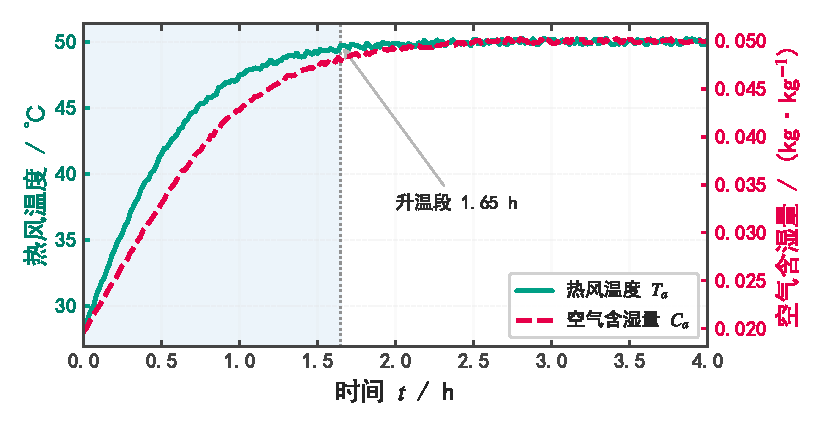
\includegraphics[width=0.9\textwidth,height=0.8\textheight,keepaspectratio]{../figures/fig_env_driving.pdf}
  \caption{附件1 热风温度与空气含湿量的双轴时序（模型的时变边界驱动）}
  \label{fig:env_driving}
\end{figure}

图~\ref{fig:env_driving} 与表~\ref{tab:data_stats} 显示，热风温度在约 $0.5\,\mathrm{h}$ 内由
$28\,^{\circ}\mathrm{C}$ 升至并稳定在 $50\,^{\circ}\mathrm{C}$ 附近（均值 $47.2\,^{\circ}\mathrm{C}$），空气含湿量
均值约 $0.045$；附件1 仅覆盖前 $4\,\mathrm{h}$，而达标需数十小时，故对 $t>4\,\mathrm{h}$ 采用
"保持末值"作为基准外推，其影响在第\ref{sec:sens}节量化（不足 $0.6\%$）。由于内部各点中
\textbf{轴心含水率最高、下降最慢}（图~\ref{fig:field_heatmap_p1}、\ref{fig:field_heatmap_p2} 已示），
"内部各点均达标"等价于轴心达标，故终点时刻取首次穿越
\begin{equation}\label{eq:endpoint}
t^{*}=\inf\Big\{t:\ \max_{0\le r\le R_0}C(r,t)<C_{\mathrm{th}}\Big\}
     =\inf\Big\{t:\ C(0,t)<C_{\mathrm{th}}\Big\},
\end{equation}
并在跨越阈值的相邻两输出步之间对 $C(0,t)$ 作线性插值定位 $t^*$，避免受输出步长限制。

\subsection{结果与分析}

图~\ref{fig:drying_curve} 给出中心与表面含水率的干燥曲线及阈值首次穿越。

\begin{figure}[H]
  \centering
  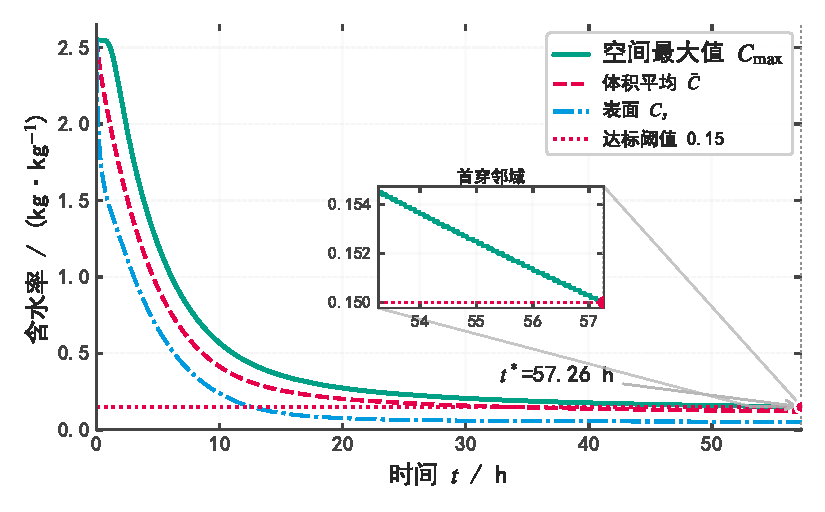
\includegraphics[width=0.9\textwidth,height=0.8\textheight,keepaspectratio]{../figures/fig_drying_curve.pdf}
  \caption{问题3 中心/表面含水率干燥曲线与达标阈值 $C_{\mathrm{th}}=0.15$ 的首次穿越}
  \label{fig:drying_curve}
\end{figure}

\begin{sloppypar}
由图~\ref{fig:drying_curve}，轴心含水率在 $t^{*}=57.262\,\mathrm{h}$ 首次降到
$C_{\mathrm{th}}=0.15$（此刻 $\max_r C=0.14999515$，前一输出步为 $0.15001272$），此时表面已降至
$0.0525$，与空气等效含水率 $C_{\mathrm{air}}\approx0.0499$ 接近但未越过，表面失水趋于平衡。
干燥曲线呈典型的\textbf{先快后慢}：初期近表面陡降，末期因 $D$ 随 $C$ 减小而拖尾。各时刻
径向剖面的堆叠演化见图~\ref{fig:ridgeline_profile}。
\end{sloppypar}

\begin{figure}[H]
  \centering
  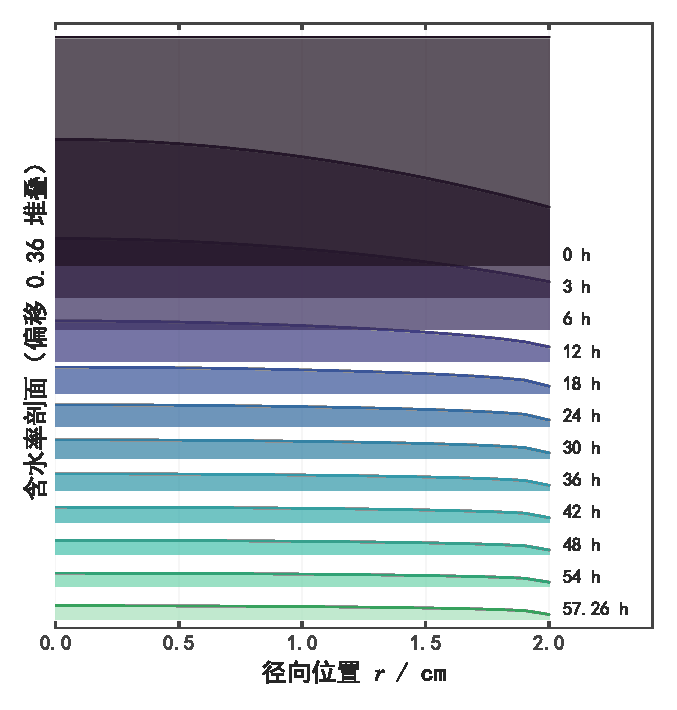
\includegraphics[width=0.8\textwidth,height=0.8\textheight,keepaspectratio]{../figures/fig_ridgeline_profile.pdf}
  \caption{问题3 各时刻径向含水率剖面的堆叠（ridgeline）演化}
  \label{fig:ridgeline_profile}
\end{figure}

图~\ref{fig:ridgeline_profile} 显示含水率剖面由初期的"表面凹陷、轴心高台"逐步整体下沉、
趋于平坦，末期全场接近 $0.15$，直观印证了达标由轴心控制。各阶段降幅见图~\ref{fig:stage_rate}。

\begin{figure}[H]
  \centering
  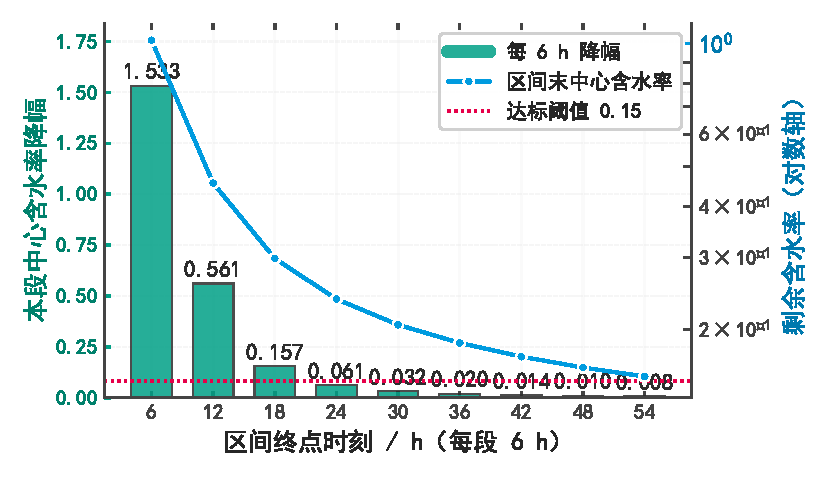
\includegraphics[width=0.9\textwidth,height=0.8\textheight,keepaspectratio]{../figures/fig_stage_rate.pdf}
  \caption{问题3 轴心含水率每 6\,h 的阶段降幅}
  \label{fig:stage_rate}
\end{figure}

图~\ref{fig:stage_rate} 把轴心含水率按每 $6\,\mathrm{h}$ 统计：前 $6\,\mathrm{h}$ 由 $2.55$ 骤降到约
$1.02$，随后各段依次为 $0.456$,\allowbreak\,$0.298$,\allowbreak\,$0.237$,\allowbreak\,$0.206$,\allowbreak\,$0.186$,\allowbreak\,$0.172$,\allowbreak\,$0.162$,\allowbreak\,$0.154$，\textbf{降幅逐段收窄}，
定量刻画了扩散受阻导致的边际效率递减——这也是干燥后段耗时占比高的根本原因。含水率时空
曲面与达标平面见图~\ref{fig:surface_3d}。

\begin{figure}[H]
  \centering
  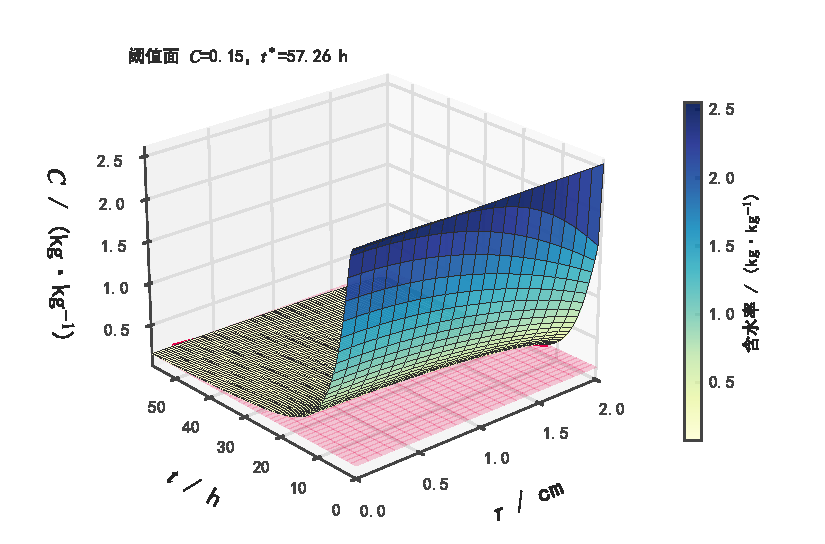
\includegraphics[width=0.9\textwidth,height=0.8\textheight,keepaspectratio]{../figures/fig_surface_3d.pdf}
  \caption{问题3 含水率 $C(r,t)$ 时空曲面与达标阈值平面的相交}
  \label{fig:surface_3d}
\end{figure}

图~\ref{fig:surface_3d} 从三维视角显示曲面与 $C=0.15$ 平面的相交线随 $t$ 由表面向轴心推进，
最后交于轴心，几何化地对应式~\eqref{eq:endpoint} 的首次穿越判据。控制机制的转换见
图~\ref{fig:biot_regime}。

\begin{figure}[H]
  \centering
  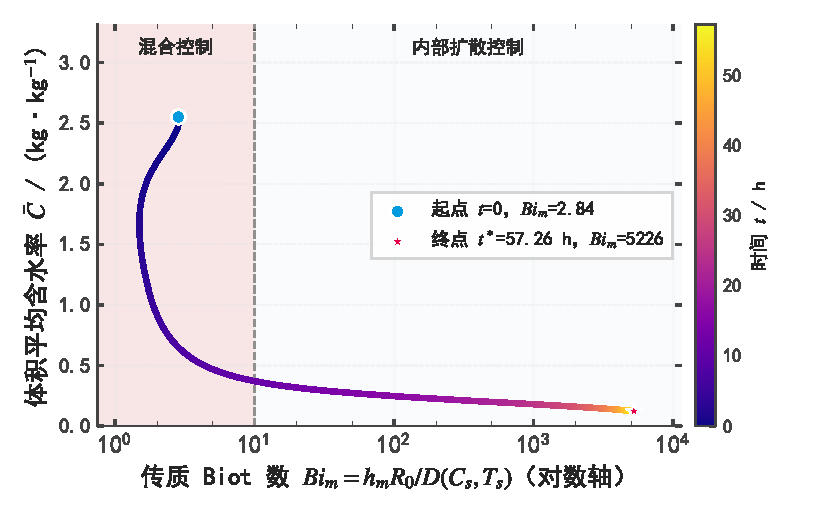
\includegraphics[width=0.9\textwidth,height=0.8\textheight,keepaspectratio]{../figures/fig_biot_regime.pdf}
  \caption{问题3 传质毕奥数 $\mathrm{Bi}_m=h_m R_0/D$ 随干燥进程的控制机制转换}
  \label{fig:biot_regime}
\end{figure}

图~\ref{fig:biot_regime} 表明 $\mathrm{Bi}_m$ 随 $D$ 减小而显著增大：初期 $\mathrm{Bi}_m\approx1.4$，
内外阻力可比；末期 $D$ 降低约一个量级使 $\mathrm{Bi}_m$ 增大到远大于 1，干燥\textbf{由外部对流控制
转为内部扩散控制}。这一转换解释了干燥曲线的拖尾，也说明单纯提高热风流速（增大 $h_m$）
在末期收益有限，改善内部扩散才是关键。
